\documentclass{beamer}

\usepackage{tikz}

%\usetheme{Madrid}

\title{
\includegraphics[scale=.5]{Git-Logo-2Color.eps}}
\author{Martin \textsc{Vassor}}

\begin{document}


\maketitle
\begin{frame}
	\frametitle{Plan}
	\tableofcontents
\end{frame}

\section{Introduction}
\subsection{Travail collaboratif}

\begin{frame}
	\frametitle{Introduction}
	\tableofcontents[currentsection]
\end{frame}

\begin{frame}
	\frametitle{Comment travailler en commun en informatique ?}
	\begin{itemize}
		\item{Autonomie/Ind\'ependance}
		\item{Modifications concurrentes}
		\item{Erreur}
	\end{itemize}
\end{frame}

\subsection{Histoire}
\begin{frame}
	\frametitle{Histoire}
	\begin{itemize}
		\item{Linus Torvalds}
		\item{D\'evelopp\'e pour Linux (remplacement BitKeeper)}
		\item{Avril 2005}
	\end{itemize}
\end{frame}

\section{Syst\`eme d\'ecentralis\'e vs. syst\`eme centralis\'e}
\subsection{Syst\`eme centralis\'e}
\begin{frame}
	\frametitle{Introduction}
	\tableofcontents[currentsection]
\end{frame}

\begin{frame}
	\frametitle{Syst\`eme centralis\'e}
	Exemple : cvs, svn
	\begin{center}
		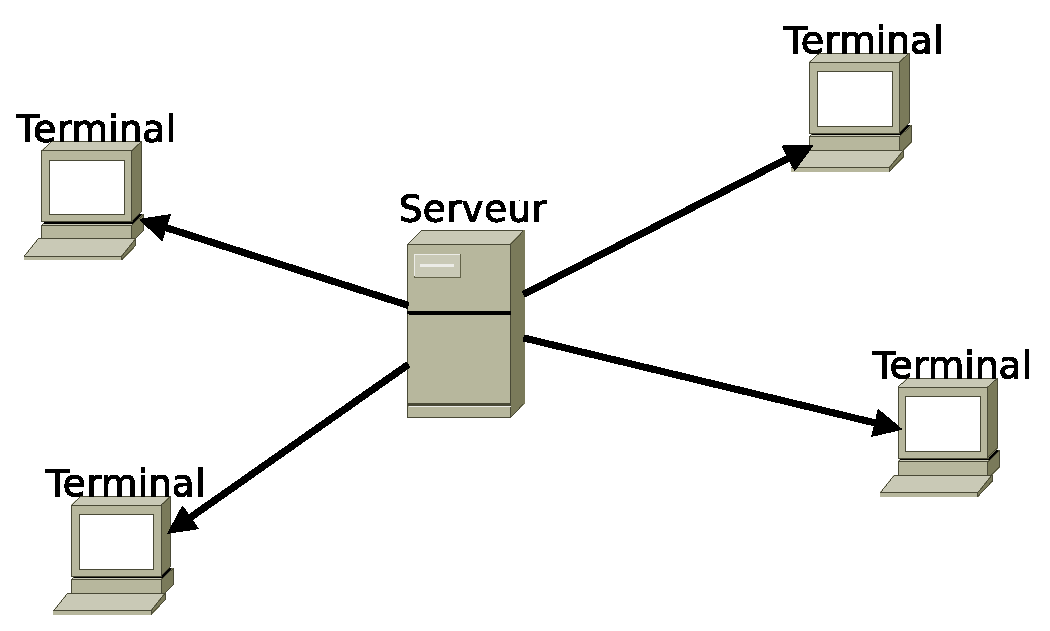
\includegraphics[scale=0.5]{Central.eps}
	\end{center}
\end{frame}

\subsection{syst\`eme d\'ecentralis\'e}
\begin{frame}
	\frametitle{Syst\`eme d\'ecentralis\'e}
	Exemple : git, mercurial
	\begin{center}
		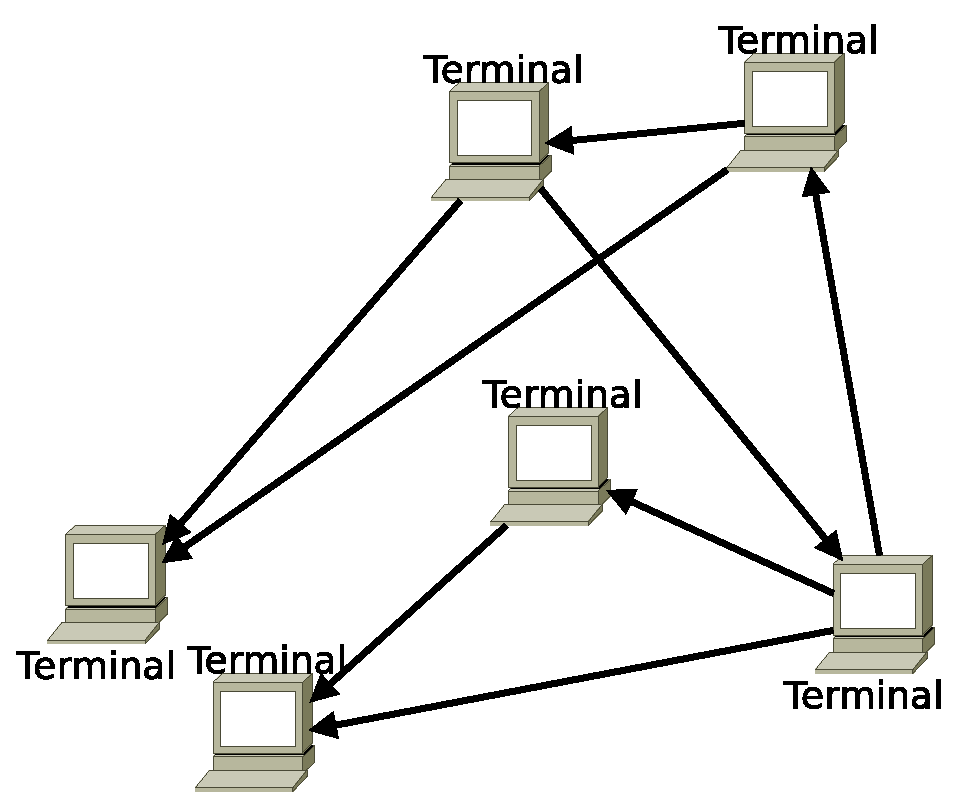
\includegraphics[scale=0.5]{Decentral.eps}
	\end{center}
\end{frame}

\section{Gestion de version}
\subsection{D\'ep\^ots}
\begin{frame}
	\frametitle{Introduction}
	\tableofcontents[currentsection]
\end{frame}
\begin{frame}
	\frametitle{D\'ep\^ots}
	\begin{enumerate}
		\item[D\'ep\^ot]{Ensemble de fichiers suivis}
	\end{enumerate}
	Syst\`eme distribu\'e : 1 utilisateur = 1 d\'ep\^ot\\
	Git : Enregistre l'\'etat du d\'ep\^ot\footnote{On peut imaginer git comme un filesystem}
\end{frame}

\subsection{\'Etats des fichiers} % untrack, unmodified, modified, staged
\begin{frame}
	\frametitle{\'Etats des fichiers}
	\begin{itemize}
		\item{untrack}
		\item{unmodified}
		\item{modified}
		\item{staged}
	\end{itemize}
\end{frame}
\subsection{Workflows/Branches}
\begin{frame}
	\frametitle{Workflows/Branches}
	Avoir plusieurs \'etats diff\'erents des fichiers.\\
	Permet le travail concurrent.
\end{frame}
\begin{frame}
	\frametitle{Workflows/Branches}
	\begin{center}
		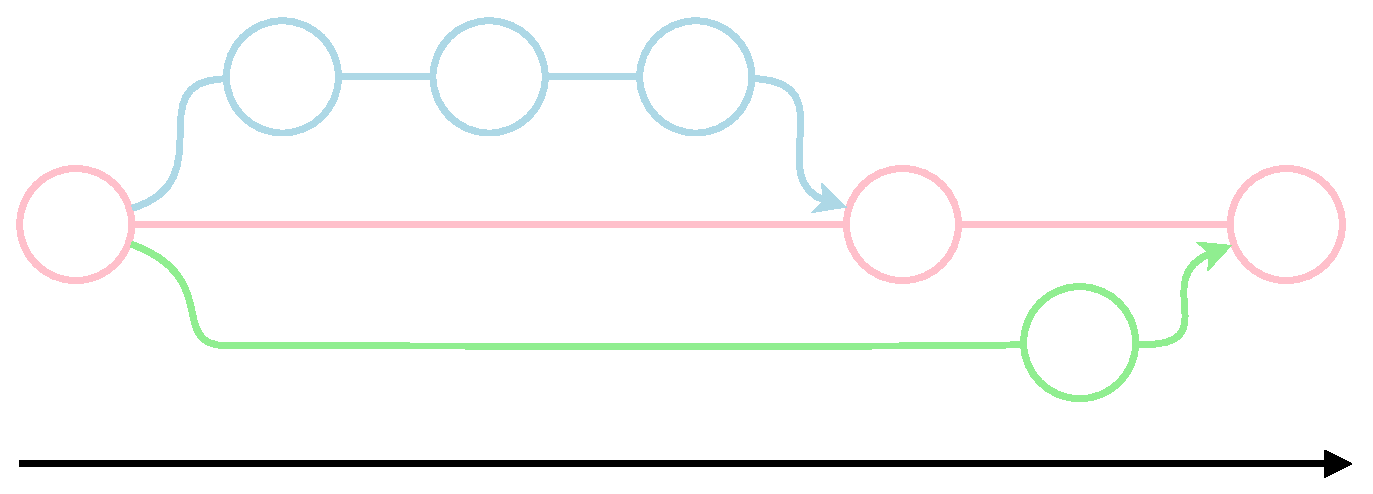
\includegraphics[scale=0.5]{Branches.eps}
	\end{center}
\end{frame}

\subsection{Fusions de branches}

\section{Github}
\subsection{Travail personnel}
\begin{frame}
	\frametitle{Travailler avec github - Travail personnel}
	\begin{itemize}
		\item{git clone https://github.com/username/reponame.git}
		\item{git add remote [remoteName] [remoteURL]}
		\item{git fetch [remote]}
		\item{git push [remoteName] [branchName]}
	\end{itemize}
\end{frame}

\subsection{Travail collaboratif}
\begin{frame}
	\frametitle{Travailler avec github - Travail collectif}
	\begin{itemize}
		\item{Cloner depuis le compte manager}
		\item{Pousser la branche sur notre compte}
		\item{Cr\'eer une \emph{pull request}}
	\end{itemize}
\end{frame}

\section{Bibliographie et ressources}
\begin{frame}
	\frametitle{Bibliographie et ressources}
	\begin{itemize}
		\item{http://git-scm.com}
		\item{https://help.github.com}
	\end{itemize}
\end{frame}
\end{document}
